
%(BEGIN_QUESTION)
% Copyright 2014, Tony R. Kuphaldt, released under the Creative Commons Attribution License (v 1.0)
% This means you may do almost anything with this work of mine, so long as you give me proper credit

Finn spenningen i forhold til jord for hvert av punktene \textbf{A} og \textbf{B} i kretsen under. 
Kretsen kan være i fire ulike tilstander: begge brytere av, bryter A på og B av, bryter A av og B på, og begge på. Du må finne spenningene for alle tilstandene.

$$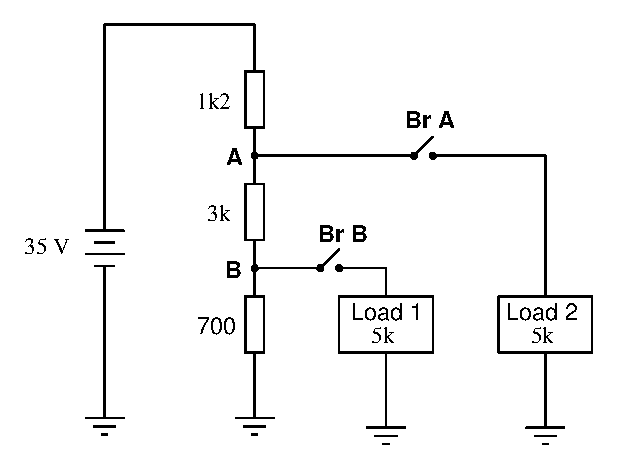
\includegraphics[width=15.5cm]{i01133x01.eps}$$

% No blank lines allowed between lines of an \halign structure!
% I use comments (%) instead, so that TeX doesn't choke.

$$\vbox{\offinterlineskip
\halign{\strut
\vrule \quad\hfil # \ \hfil & 
\vrule \quad\hfil # \ \hfil & 
\vrule \quad\hfil # \ \hfil & 
\vrule \quad\hfil # \ \hfil & 
\vrule \quad\hfil # \ \hfil \vrule \cr
\noalign{\hrule}
%
% First row
Spenning & Begge laster av & Last 1 på (kun) & Last 2 på (kun) & Begge laster på \cr
%
\noalign{\hrule}
%
% Second row
$U_A$ &  &  &  &  \cr
%
\noalign{\hrule}
%
% Third row
$U_B$ &  &  &  &  \cr
%
\noalign{\hrule}
} % End of \halign 
}$$ % End of \vbox

\underbar{file i01133}
%(END_QUESTION)





%(BEGIN_ANSWER)

$$\vbox{\offinterlineskip
\halign{\strut
\vrule \quad\hfil # \ \hfil & 
\vrule \quad\hfil # \ \hfil & 
\vrule \quad\hfil # \ \hfil & 
\vrule \quad\hfil # \ \hfil & 
\vrule \quad\hfil # \ \hfil \vrule \cr
\noalign{\hrule}
%
% First row
Spenning & Begge laster av & Last 1 på (kun) & Last 2 på (kun) & Begge laster på \cr
%
\noalign{\hrule}
%
% Second row
$V_A$ & 26.4 volt & 26.3 volt & 22.4 volt & 22.3 volt \cr
%
\noalign{\hrule}
%
% Third row
$V_B$ & 5 volt & 4.46 volt & 4.23 volt & 3.78 volt \cr
%
\noalign{\hrule}
} % End of \halign 
}$$ % End of \vbox

%(END_ANSWER)





%(BEGIN_NOTES)

Elevene må vurdere (og eventuelt tegne om) kretsen for hver lasttilstand, som er et av hovedpoengene i denne oppgaven.  At en krets kan ``endre seg'' bare ved å slå en bryter, er et viktig konsept for elektronikkelever å forstå.  

Et annet konsept i denne oppgaven er spenninger oppgitt i enkeltpunkter med implisitt referanse til jord.  Vis elevene hvordan hver spenning bare er referert med én bokstav, enten {\bf A} eller {\bf B}.  Det finnes selvsagt ikke noe som heter spenning i ett enkelt punkt i en krets, så vi trenger et referansepunkt, og her er det jord.  Dette er {\it svært} vanlig i elektroniske kretser av alle typer, og er nyttig å bli eksponert for tidlig i elektronikkutdanningen.

Et mindre åpenbart poeng i oppgaven er å introdusere begrepet diskrete tilstander (lasttilstander) som følger av et gitt antall boolske elementer (brytere).  Med to lastbrytere finnes fire mulige lasttilstander i kretsen, som er en forsmak på binære tilstander i digitale kretser.

%INDEX% Elektronikkrepetisjon: serie-parallellkretser

%(END_NOTES)

